%_____________________________________________________________________________________________
% Chapter 5: Implementation
%_____________________________________________________________________________________________

\chapter{Implementation}
\label{ch:impl}

\section{Tools and Technologies}
The system is written in Python. Models, auxiliary models and domain classifiers use scikit-learn~\cite{pedregosa2011sklearn}; statistics use NumPy and SciPy; tables use pandas; figures use matplotlib; and the dashboard uses Streamlit with Altair charts. Datasets are downloaded from OpenML~\cite{vanschoren2014openml}. The code is version-controlled with git and hosted on GitHub, where GitHub Actions runs linting, tests and a benchmark gate on every push. Diagrams were drawn with draw.io, and the paper and this report were typeset in \LaTeX.

\section{Development History: Ten Versions}
The final design was reached in ten versions (\figref{fig:evolution}). Versions v1--v5 were exploratory: they used synthetic scenarios and natural streams and were analysed after the fact. Versions v6--v10 were pre-registered (Section~\ref{sec:prereg}). Each version started from what had gone wrong in the previous one. Earlier results were kept as published.

\begin{figure}[H]
\centering
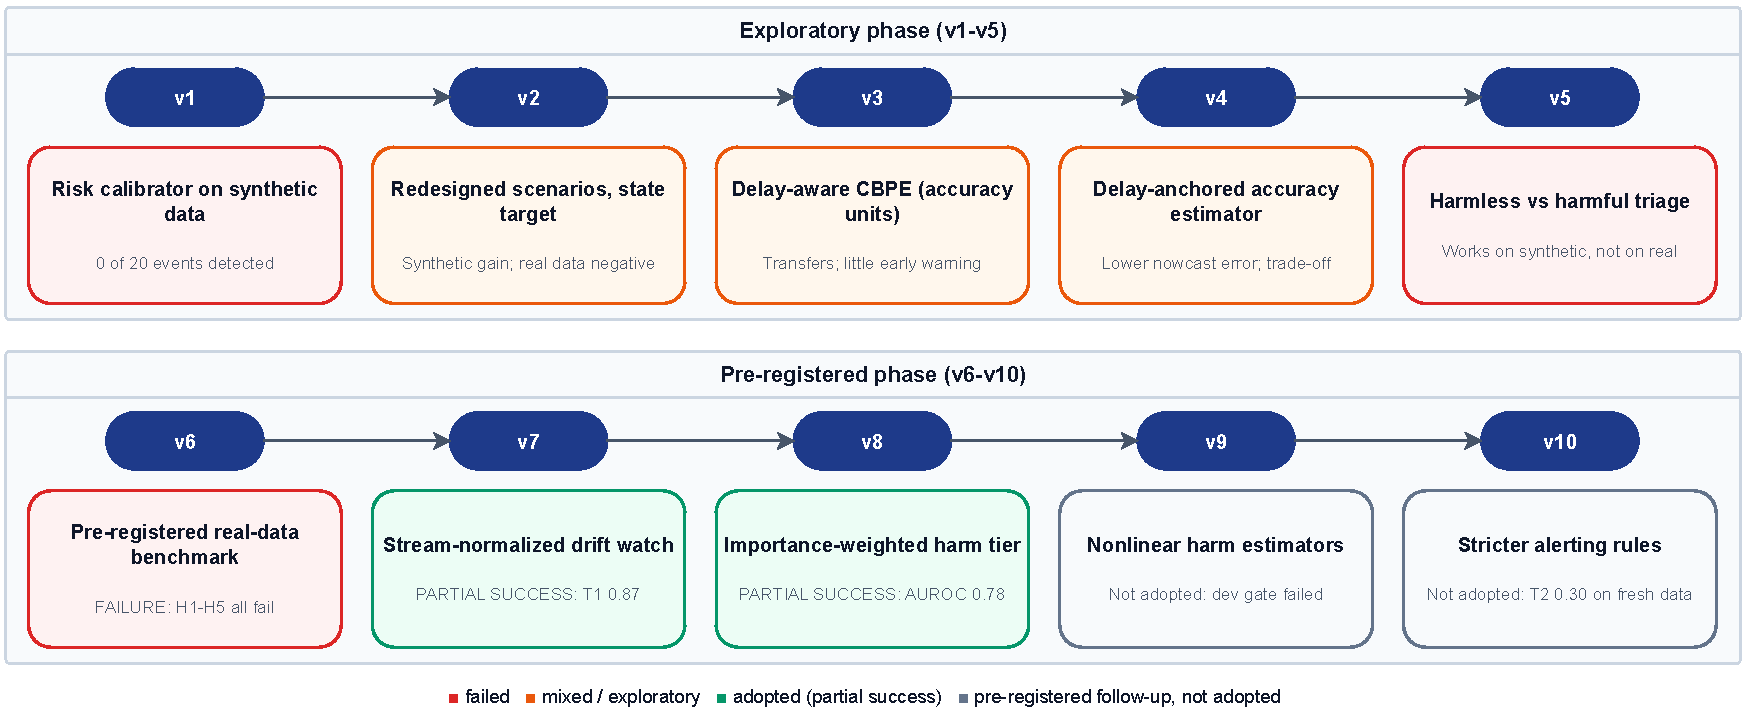
\includegraphics[width=\textwidth]{fig_evolution.pdf}
\caption{The ten versions of the system and what each showed.}
\label{fig:evolution}
\end{figure}

\subsection{v1: the original prototype's risk calibrator}
\label{sec:v1}
The first evaluation used controlled synthetic episodes (clean, harmless shift, gradual and abrupt harmful shift) with seeds split into training, validation and test groups, and label delays of 0, 2 and 5 batches. On 120 held-out episodes the learned risk calibrator matched \textbf{0 of 20} harmful events at every delay, while the fixed DEWS drift score matched 9 of 20, all after the event had started. We traced the failure to two design errors. In all 50 seeds the accuracy fell in the same batch as the intervention, so no monitor could have warned early. And the risk target (``an event \emph{starts} in the next 5 batches'') marked every batch after onset as negative, so the calibrator learned that more drift meant less risk.

\subsection{v2: redesigned scenarios and a state target}
\label{sec:v2}
v2 introduced noisy labels (baseline accuracy about 0.78), a randomised onset, relevant and nuisance features, a state target (``a degraded run starts or continues within the next 5 batches''), and a baseline that simply waits for delayed labels. On 250 held-out synthetic episodes the signals-only calibrator warned before onset in 98\% of harmful gradual episodes, about 4 batches ahead, where the fixed DEWS score gave no early warning (\tabref{tab:v2}). A leave-one-dataset-out study on four natural streams (electricity, airlines, covertype, bank-marketing), however, was negative: drift signals ranked accuracy risk weakly, and every signal-based threshold that met the budget on the other datasets raised 4--16 times more false alerts on the held-out one.

\begin{table}[H]
\caption{v2 controlled study, label delay $L=2$, 250 held-out synthetic episodes.}
\label{tab:v2}
\centering
\small
\begin{tabular}{@{}lcccc@{}}
\toprule
Method & Recall & Early-warning rate & AUROC & Brier \\
\midrule
Fixed DEWS score & 0.00 & 0.00 & 0.56 & -- \\
Confidence only & 0.44 & 0.27 & 0.50 & -- \\
Wait for delayed labels & 1.00 & 0.42 & 0.90 & -- \\
Calibrator, signals only & 0.73 & 0.42 & 0.83 & 0.161 \\
Calibrator, signals + matured accuracy & 1.00 & 0.56 & 0.94 & 0.086 \\
\bottomrule
\end{tabular}
\end{table}

\subsection{v3: delay-aware confidence-based estimation}
v3 expressed the score in accuracy units, which is what the event rule itself uses. It estimates each batch's accuracy as the mean top-class probability (as in CBPE) and corrects the bias with the residual of the latest 5 batches whose labels have already arrived. On four unseen natural streams this delay-aware CBPE stayed at 0.3--7 false alerts per 100 clean batches, against 10--11 for the drift scores, a first sign that units matter. It did not, however, give more early warning than waiting for labels.

\subsection{v4: delay-anchored accuracy estimation}
v4 anchored the estimate on the last matured accuracy and corrected it with a ridge regression on the change in 11 label-free signals, including disagreement with auxiliary models trained on the same reference rows. Disagreement turned out to be the most informative label-free error signal (mean within-window Spearman correlation 0.41 with error, against 0.19 for confidence drop). The estimator reduced nowcast error compared with stale labels, increasingly with delay (\figref{fig:nowcast}), but against waiting for labels it was a trade-off rather than a win.

\begin{figure}[H]
\centering
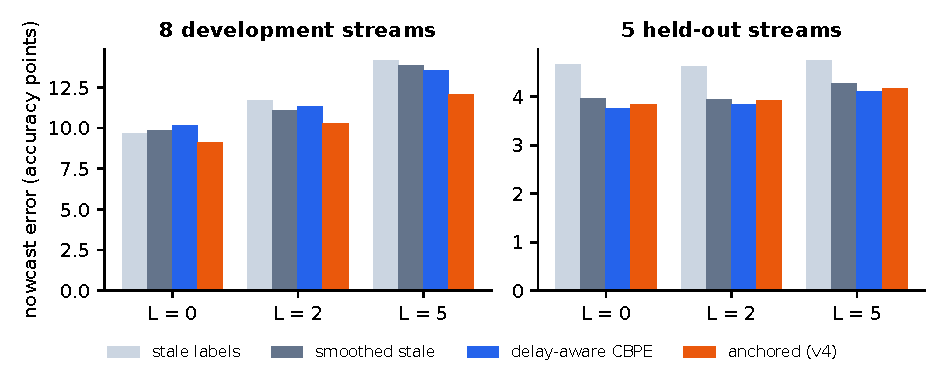
\includegraphics[width=\textwidth]{ch_v4_nowcast.pdf}
\caption{v4 accuracy nowcast error (mean absolute error in accuracy points) on 8 development streams (leave-one-dataset-out) and 5 held-out streams, by label delay.}
\label{fig:nowcast}
\end{figure}

\subsection{v5: harmless versus harmful shifts}
v5 asked whether the monitor could tell harmful from harmless shifts. A relevance-weighted shift, $\sum_j \text{importance}_j\cdot\mathrm{KS}_j$, separated them perfectly on synthetic data (AUROC 1.0), where harmlessness meant ``this feature does not matter''. On 13 real streams it did not (AUROC 0.53 on held-out streams). A sustained-alert rule did not help either. This is why v6 moved to real data with a pre-registered protocol.

\subsection{v6--v10: pre-registered experiments}
v6 built the re-sampling benchmark of Section~\ref{sec:benchmark} and evaluated a delay-aware risk calibrator under a full pre-registered protocol. It failed, and its diagnosis (thresholds in raw units do not transfer) led to the stream-normalised drift watch of v7. v7's second tier failed to separate harm, which led to the reference-based harm tier of v8. v9 and v10 tried to improve the harm tier and were not adopted. The results are reported in Chapter~\ref{ch:results}.

\section{Code Structure}
\tabref{tab:code} lists the main modules of the final system.

\begin{table}[H]
\caption{Main modules of the code base.}
\label{tab:code}
\centering
\small
\begin{tabularx}{\textwidth}{@{}p{5.3cm}X@{}}
\toprule
Module & Responsibility \\
\midrule
\texttt{dews/resample\_benchmark.py} & builds benchmark episodes from real datasets (Algorithm~\ref{alg:episode}) \\
\texttt{dews/v6\_signals.py} & per-batch signal extraction with each episode's monitored model and auxiliary models \\
\texttt{dews/v6\_eval.py} & event rule, warning tiers, false alerts, AUROC, threshold selection, v6 calibrator \\
\texttt{dews/v7\_monitor.py} & robust normalisation and the drift-watch score \\
\texttt{dews/harm\_estimation.py} & importance-weighted reference accuracy and the harm score \\
\texttt{dews/v6/v7/v8\_config.py} & frozen protocols: datasets, seeds, hypotheses, pass rules \\
\texttt{dews/detection.py}, \texttt{monitoring.py} & original DEWS detectors (KS, PSI, JSD, MMD, confidence) and fused score \\
\texttt{dews/v2.py}, \texttt{anchored.py} & exploratory library (v2--v4), delay-anchored estimator \\
\texttt{scripts/run\_v6\_*.py}, \texttt{run\_v7.py}, \texttt{run\_v8.py} & development, freezing, download, extraction and one-time confirmation \\
\texttt{scripts/make\_verdict.py} & applies the v6 pass rules and writes the verdict \\
\texttt{scripts/run\_ablations.py}, \texttt{run\_posthoc.py} & ablations and post hoc baselines \\
\texttt{scripts/reproduce.py} & one-command rebuild and verification of all verdicts \\
\texttt{streamlit\_app.py}, \texttt{app\_pages/}, \texttt{dashboard/} & the dashboard \\
\texttt{tests/} & unit tests \\
\bottomrule
\end{tabularx}
\end{table}

\section{Key Implementation Details}
\subsection{Enforcing label delay}
All label-derived features are computed from a helper that receives the current batch index and the delay and returns only the accuracies of batches $b \le t-\max(L,1)$. The same rule is used by the replay in the dashboard. Unit tests change the labels of batches that have not yet matured and check that no score at time $t$ changes.

\subsection{Per-batch monitoring}
Algorithm~\ref{alg:monitor} shows the per-batch logic of the final two-tier monitor.

\begin{algorithm}[H]
\caption{Two-tier monitoring of one stream}
\label{alg:monitor}
\begin{algorithmic}[1]
\Require frozen $f$, reference $(X_R, y_R)$, thresholds $\tau_W=4.011$, $\tau_H=0.0115$, delay $L$
\State $c_i \gets \mathbb{1}[f(x_i)=y_i]$ for every reference row
\For{each batch $B_t$}
  \State compute the 7 signals $x_t^{(k)}$ from $B_t$, $f$ and the auxiliary models
  \State fit domain classifier $g_t$ on $X_R$ (label 0) versus $B_t$ (label 1)
  \State $w_i \gets \min(\rho_i/\bar\rho, 20)$; \quad $\hat a_t \gets \sum_i w_i c_i / \sum_i w_i$
  \If{$t \geq 8$}
    \State $z^{(k)}_t \gets (x^{(k)}_t - \mathrm{med}(x^{(k)}_{0:8})) / \max(1.4826\,\mathrm{MAD}(x^{(k)}_{0:8}), 0.01)$
    \State \textbf{if} $\max_k z^{(k)}_t \geq \tau_W$ \textbf{then} raise WATCH
    \State \textbf{if} $\mathrm{med}(\hat a_{0:8}) - \hat a_t \geq \tau_H$ \textbf{then} raise HARM
  \EndIf
  \State release labels of $B_{t-\max(L,1)}$; update observed accuracy; confirm or clear alerts by the event rule
\EndFor
\end{algorithmic}
\end{algorithm}

\subsection{Pre-registration in code}
Each pre-registered experiment has its own configuration module in \texttt{dews/} (for example \texttt{v7\_config.py}; the v10 module is on its branch) that defines the datasets, seeds, settings and every hypothesis with its pass rule; a unit test checks the v6 configuration. Development scripts write the chosen thresholds to \texttt{artifacts/vN/frozen\_vN.json}. The first 16 hexadecimal digits of the file's SHA-256 hash are recorded in the protocol document, and the confirmation script computes the hash again and refuses to run if it is not found there. Downloads of confirmation datasets are separate commands that were run only after this commit.

\subsection{Parallel extraction}
Signal extraction trains several models per batch and dominates the run time. Extraction runs as six independent shard processes, each writing its own result file, which are merged before evaluation. Rebuilding everything from scratch takes about two hours on the development laptop.

\section{Dashboard}
The dashboard has four pages. The \emph{Overview} (\figref{fig:scr_overview}) summarises the main results. The \emph{Live monitor} (\figref{fig:scr_live}) replays a saved episode batch by batch: the user chooses the data group, dataset, episode type and label delay, and moves a slider over the batches. Key moments are shown as metrics (shift start, accuracy event, first drift-watch alert, first harm warning, label confirmation), with both tier scores divided by their thresholds, the accuracy seen through delayed labels, the label-free harm estimate, and a breakdown of which signals moved. The \emph{Verdicts} page lists every pre-registered hypothesis with its result, and \emph{Why it works} presents the ablation findings.

\begin{figure}[H]
\centering
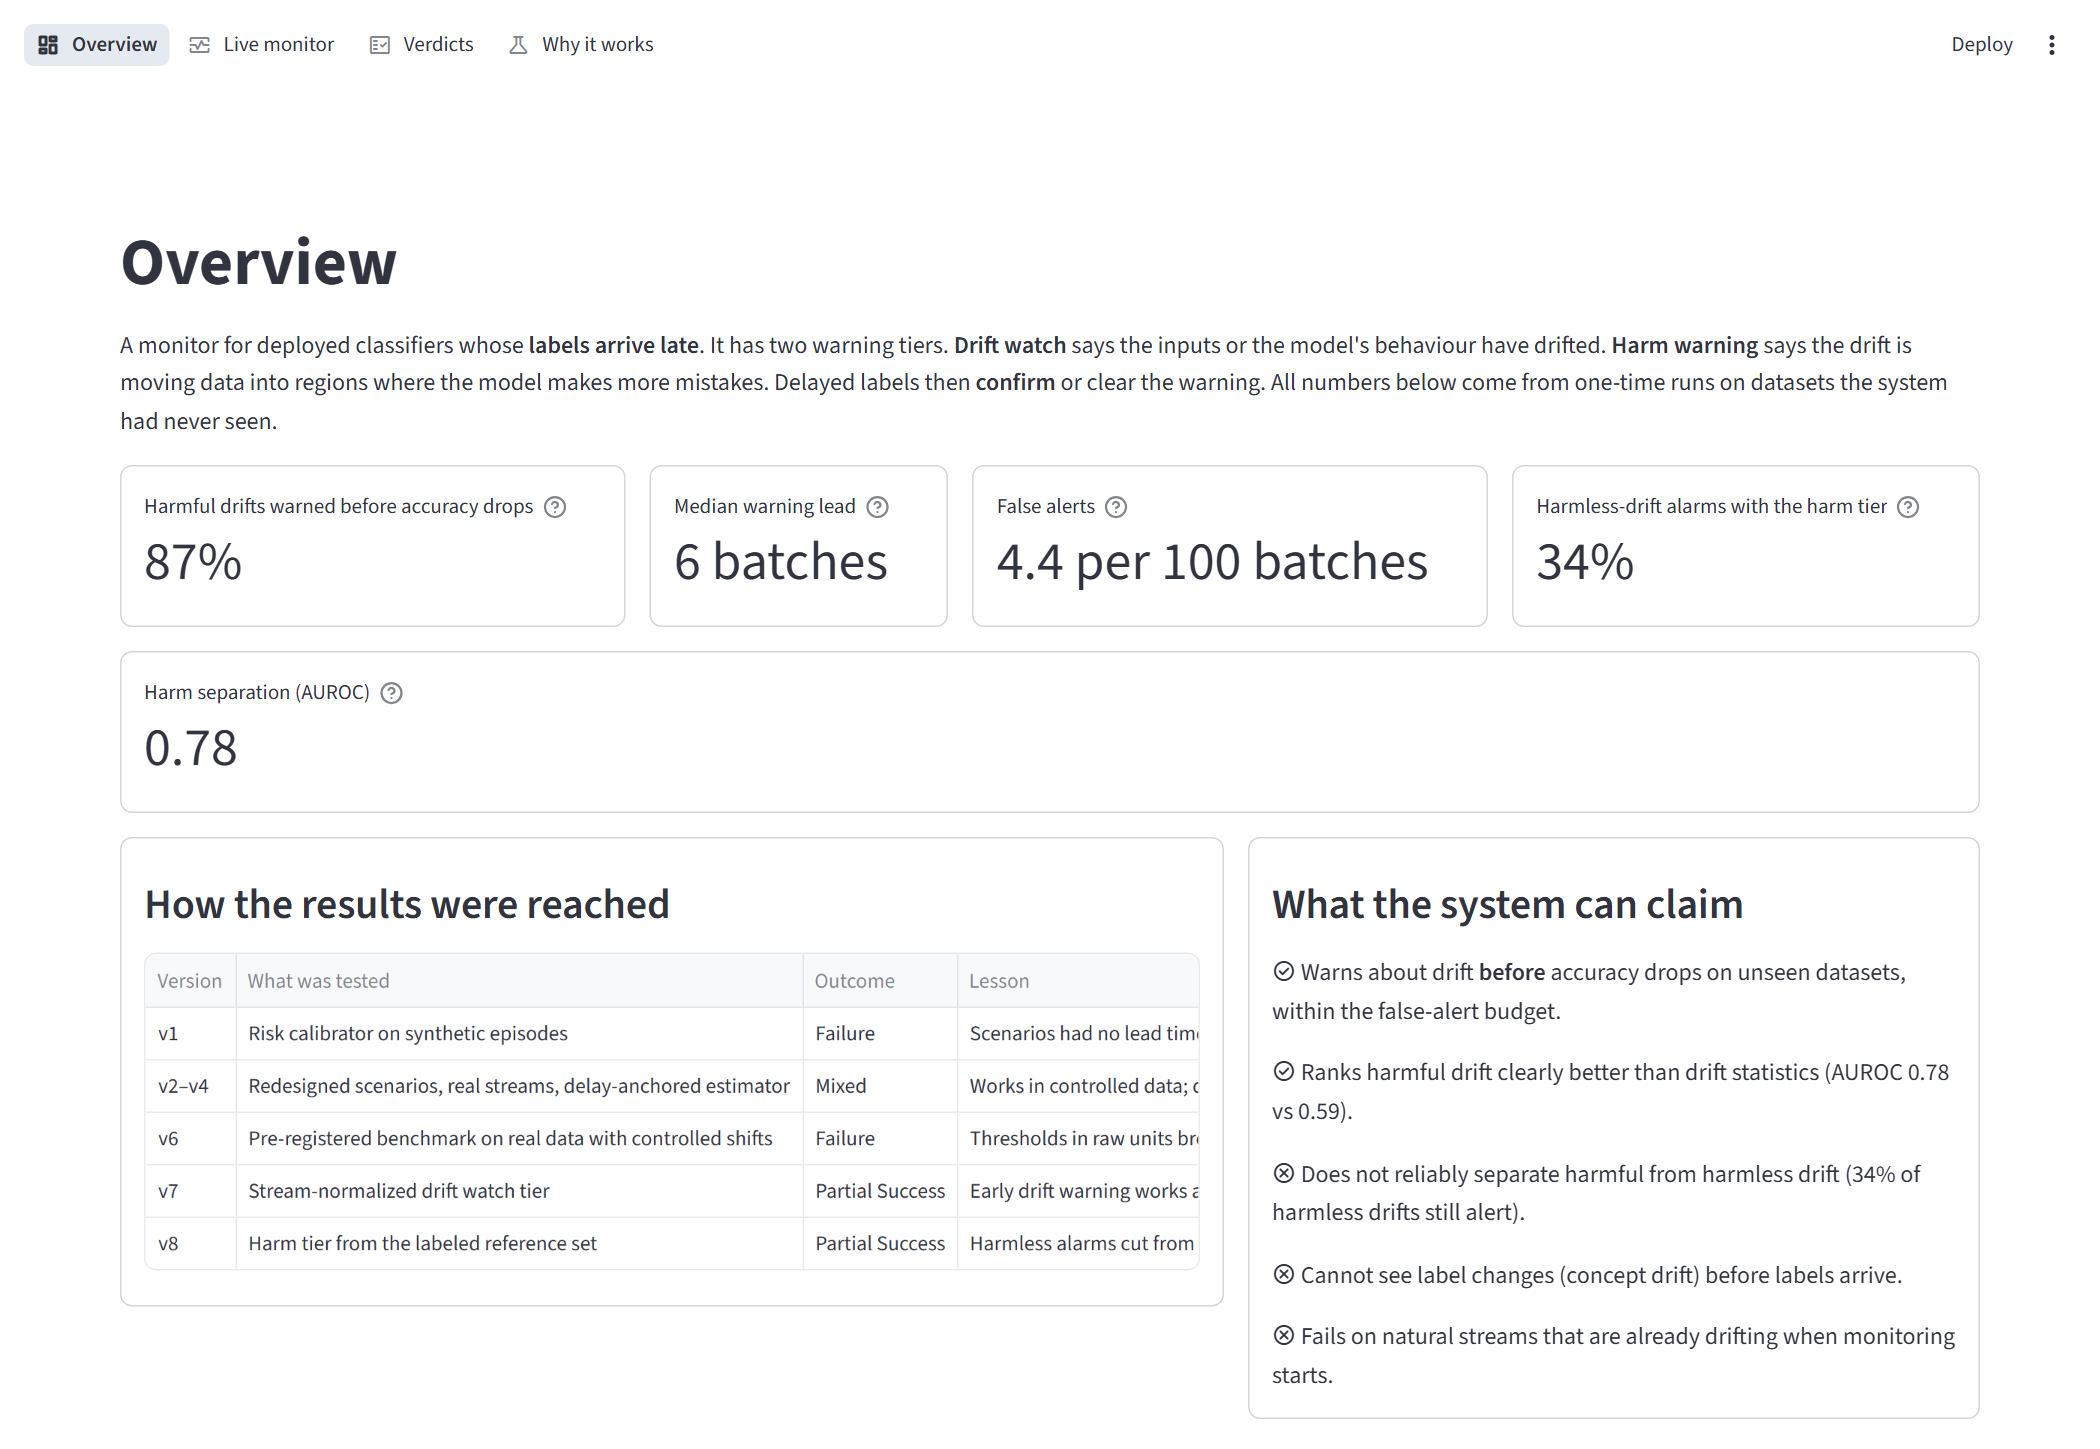
\includegraphics[width=0.92\textwidth]{overview.png}
\caption{Dashboard: Overview page.}
\label{fig:scr_overview}
\end{figure}

\begin{figure}[H]
\centering
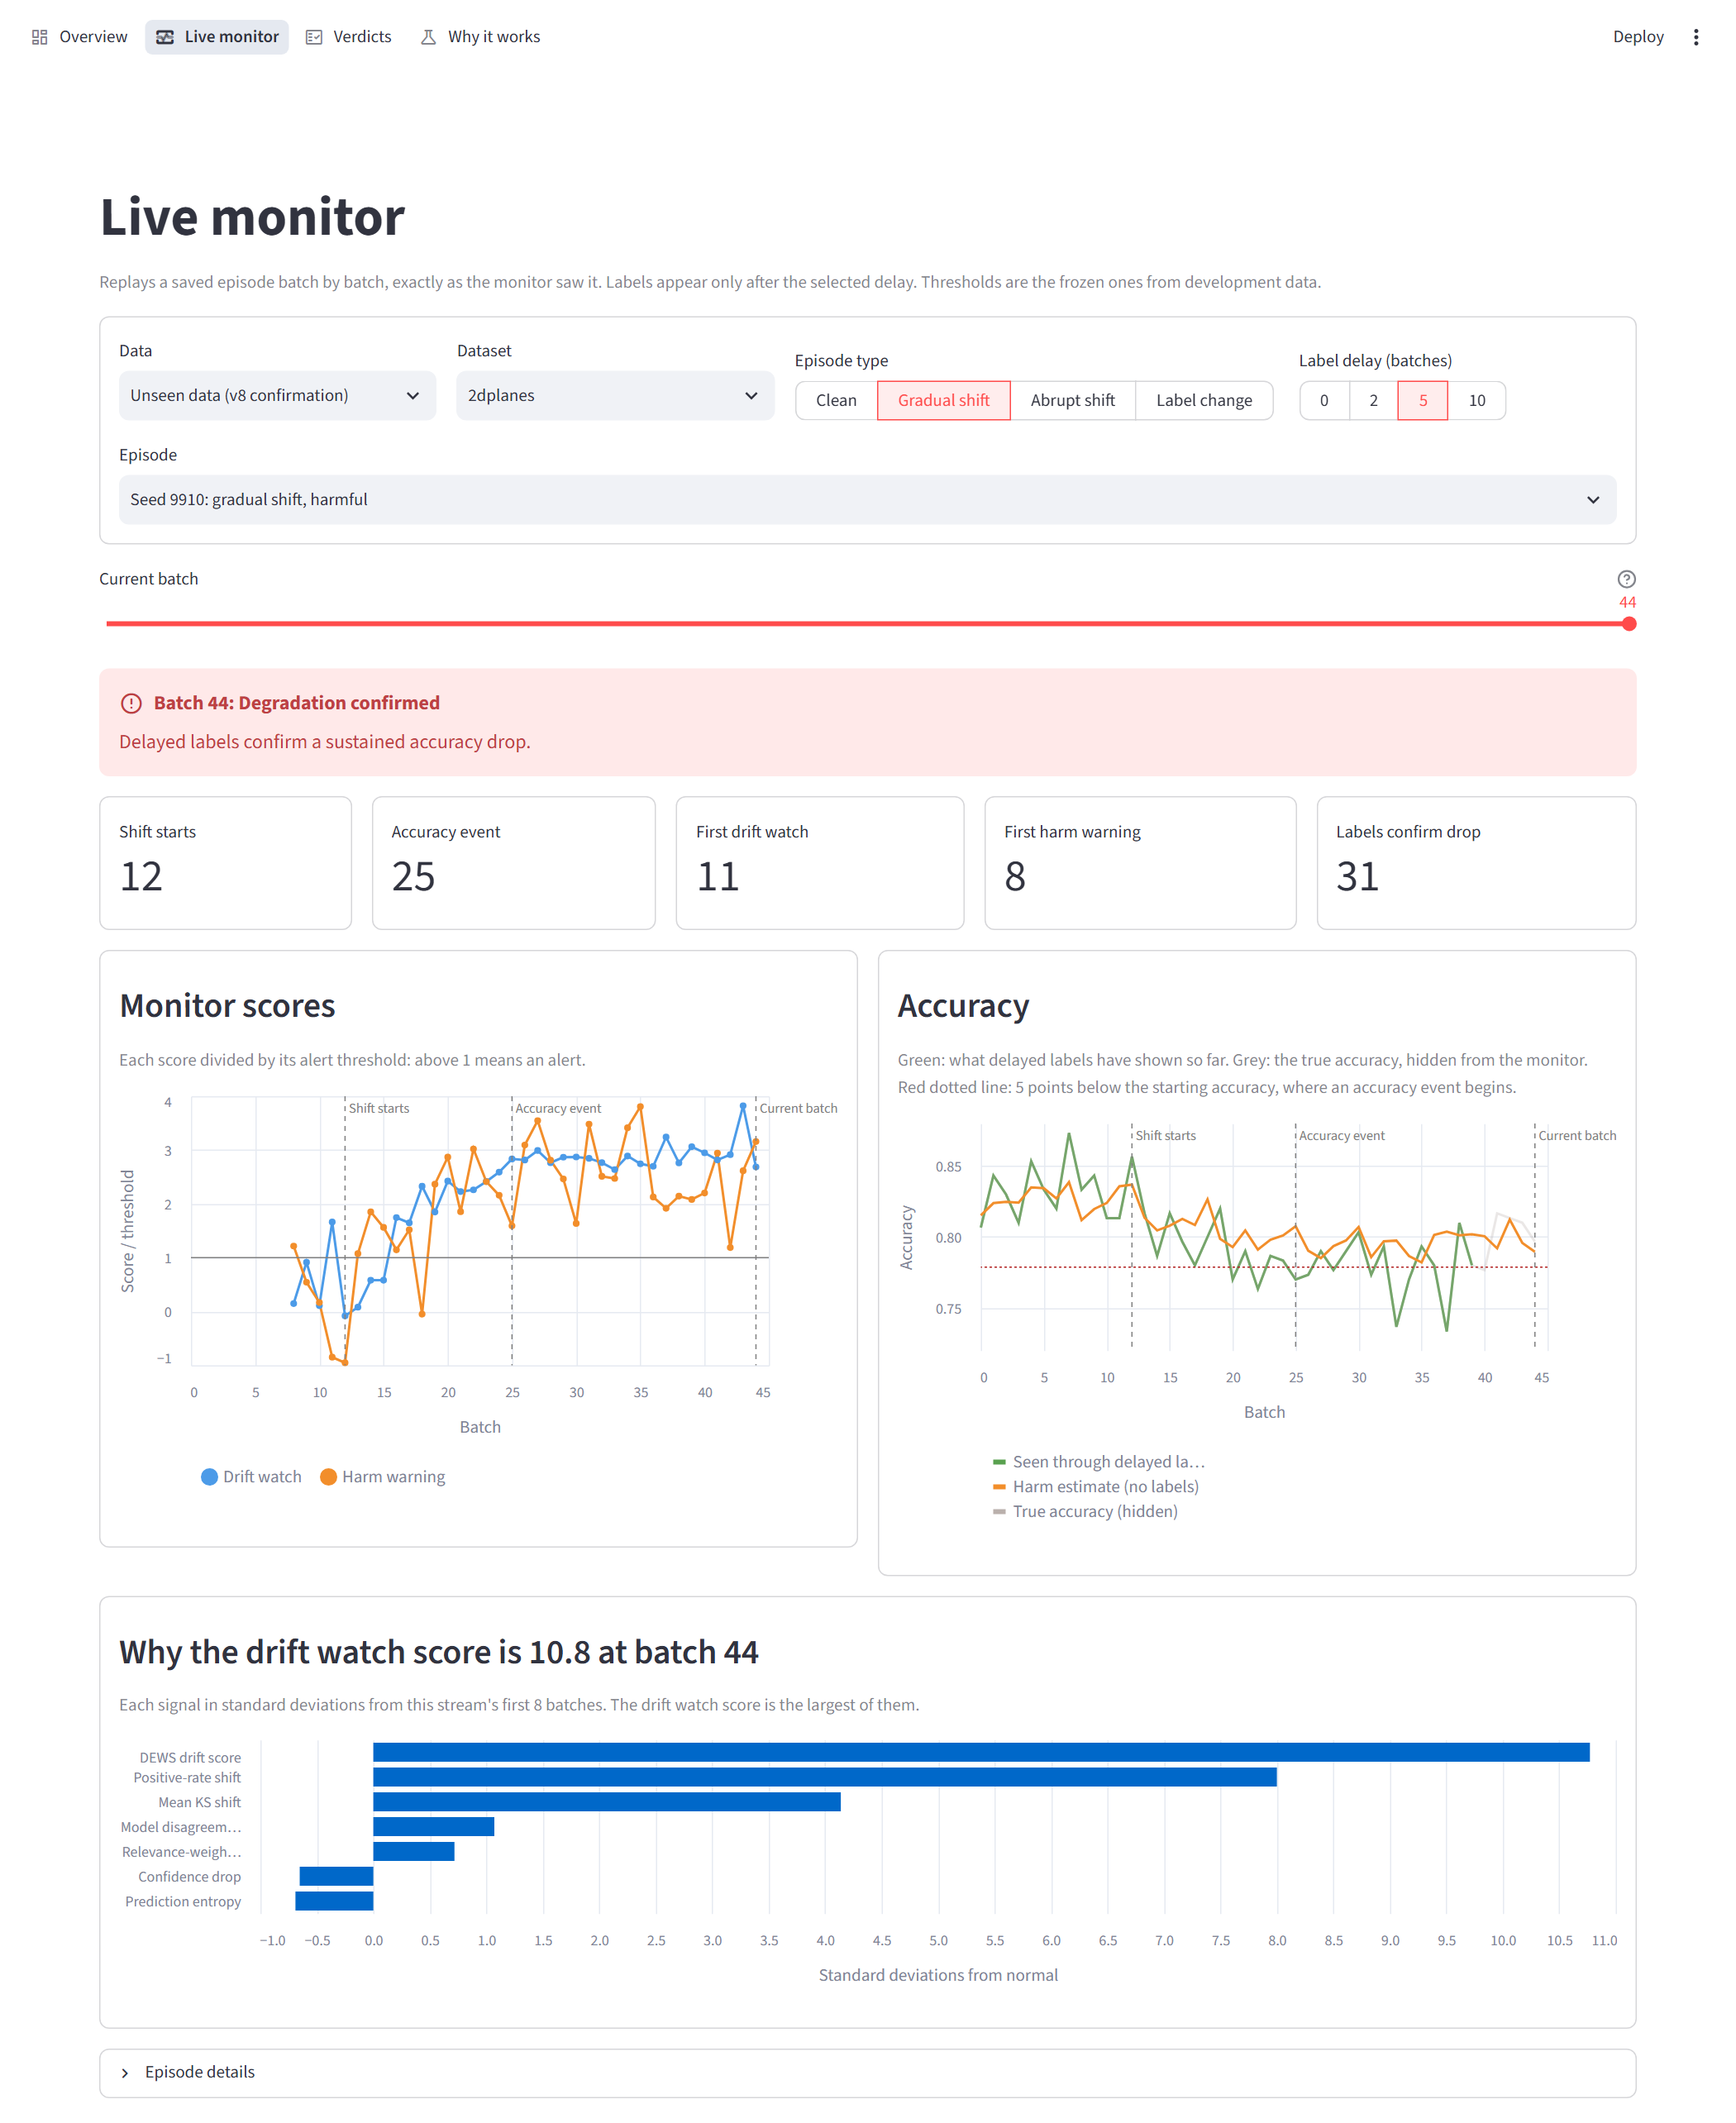
\includegraphics[width=0.8\textwidth]{live_monitor.png}
\caption{Dashboard: Live monitor replaying a harmful gradual shift on an unseen dataset (2dplanes, label delay 5). Alerts before the shift at batch 12 count as false alerts in the evaluation.}
\label{fig:scr_live}
\end{figure}

\begin{figure}[H]
\centering
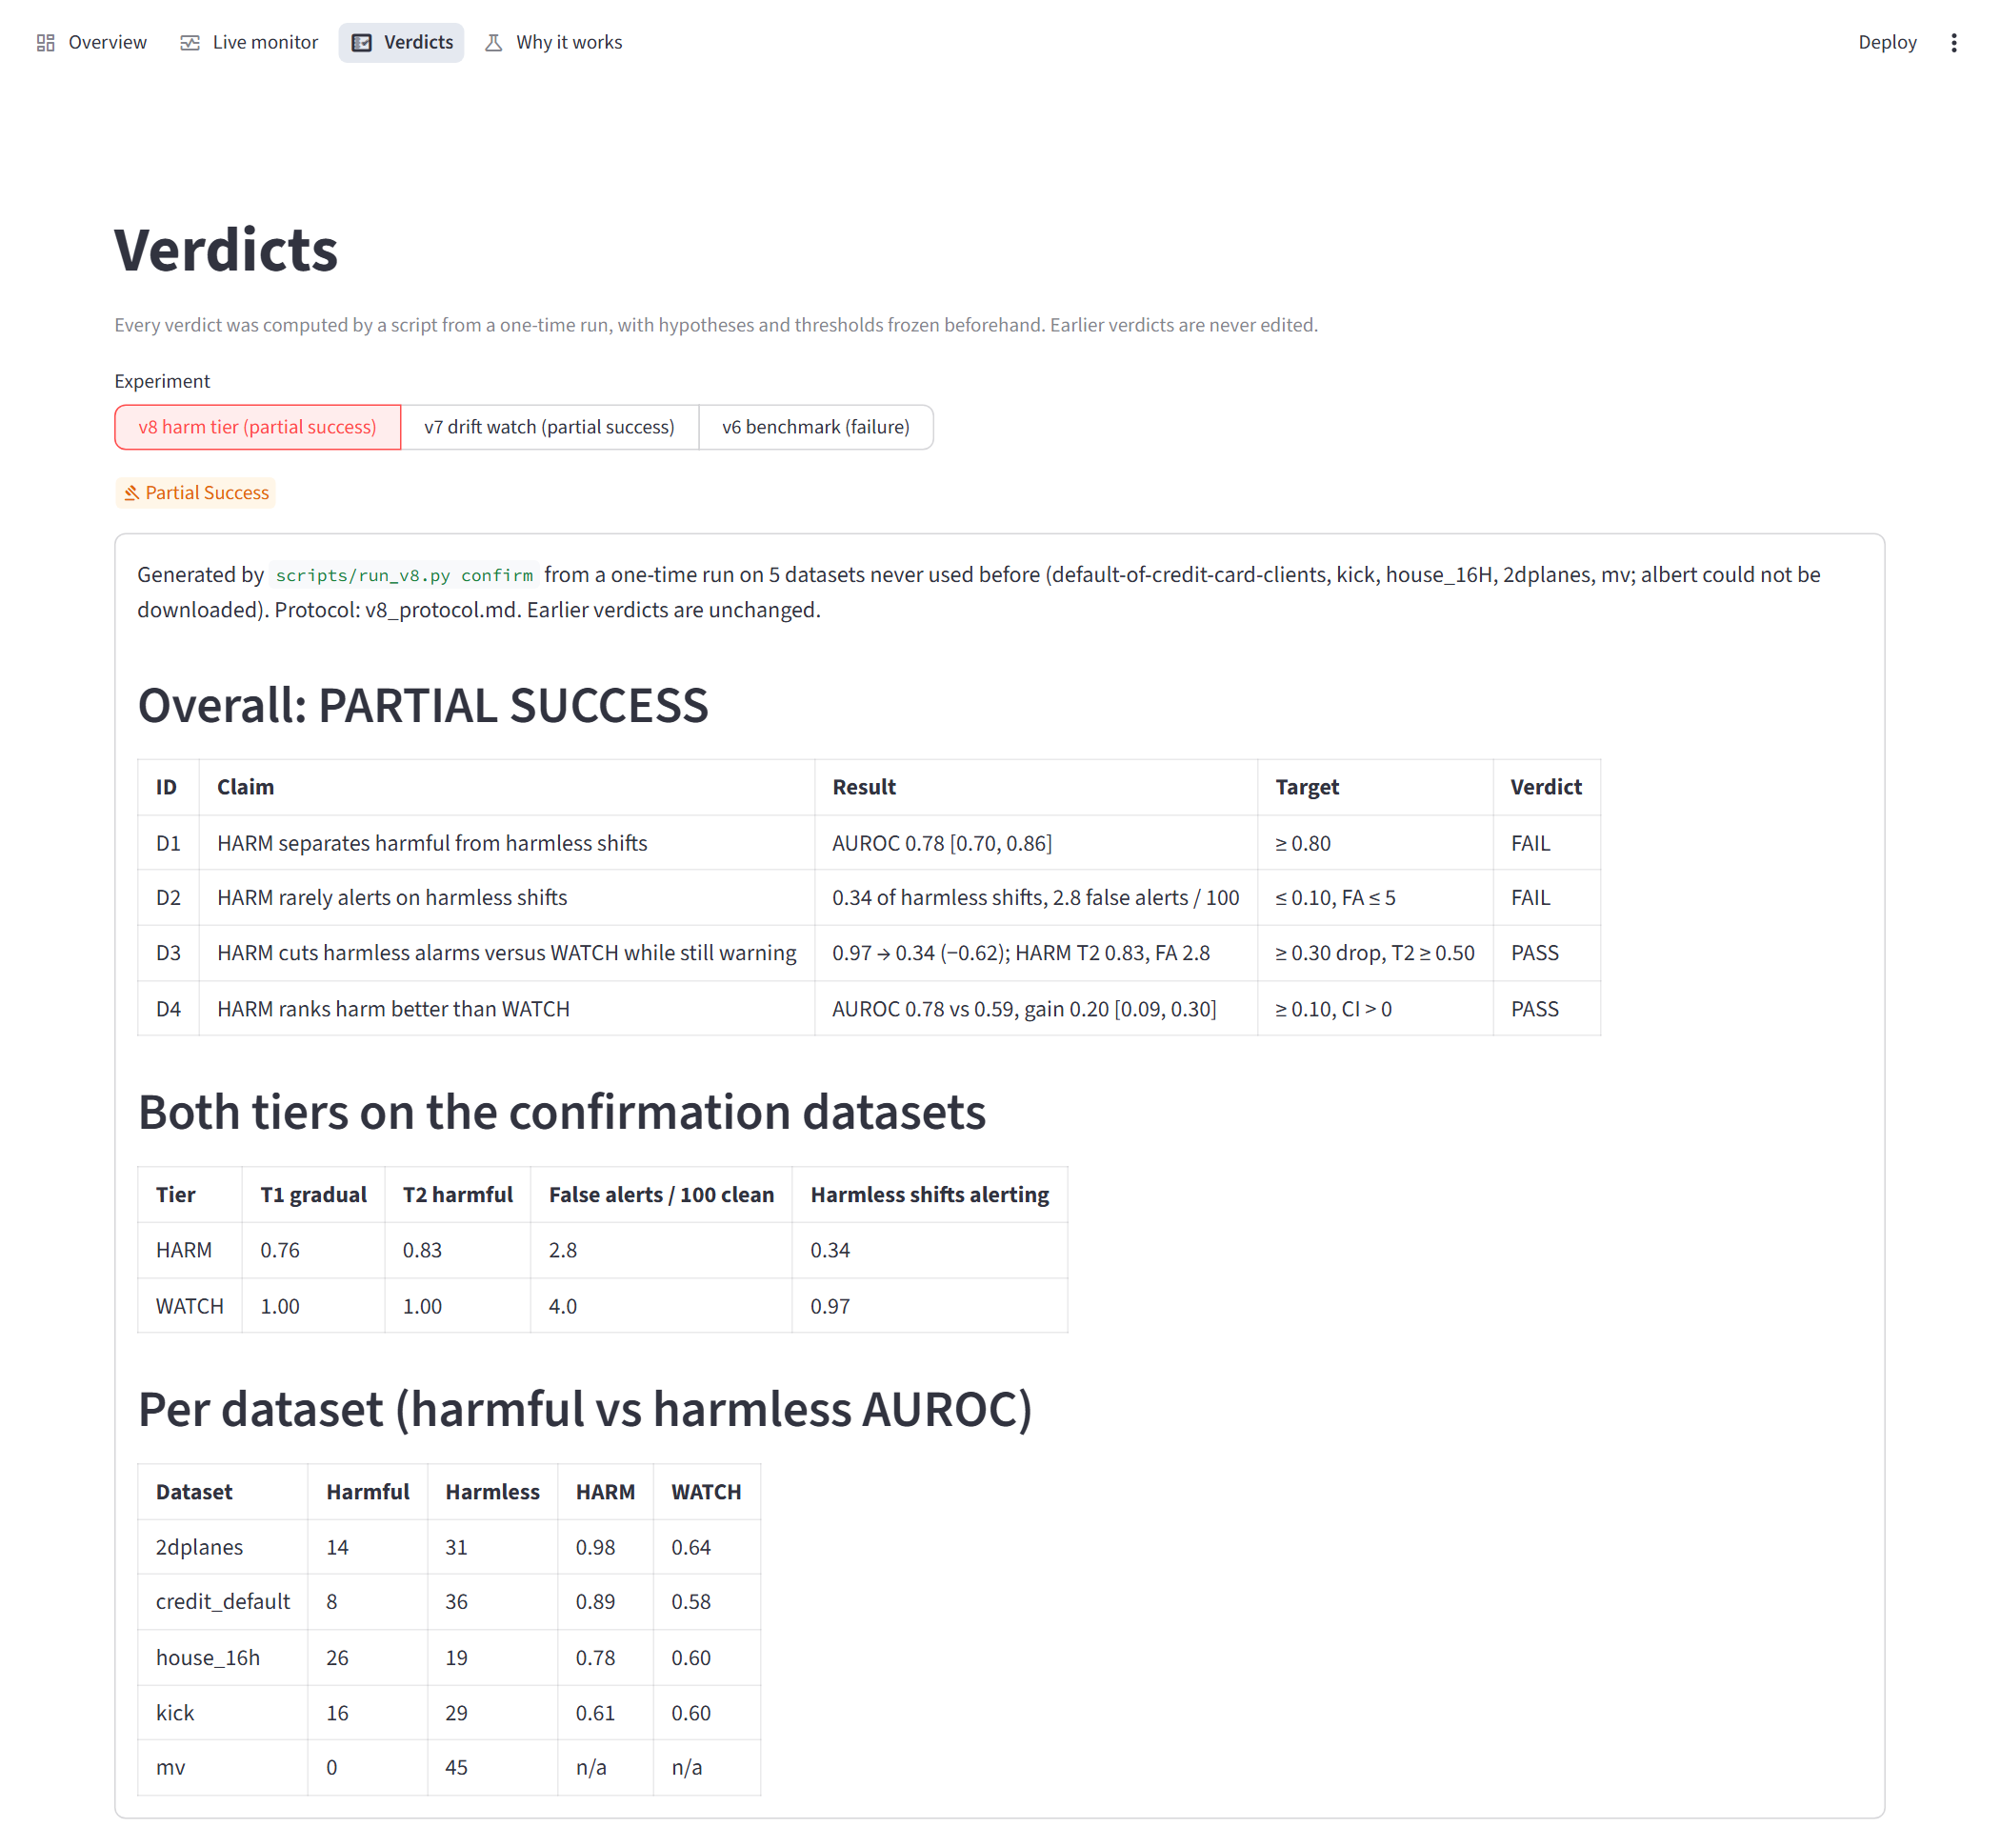
\includegraphics[width=0.85\textwidth]{verdicts.png}
\caption{Dashboard: Verdicts page.}
\label{fig:scr_verdicts}
\end{figure}

\begin{figure}[H]
\centering
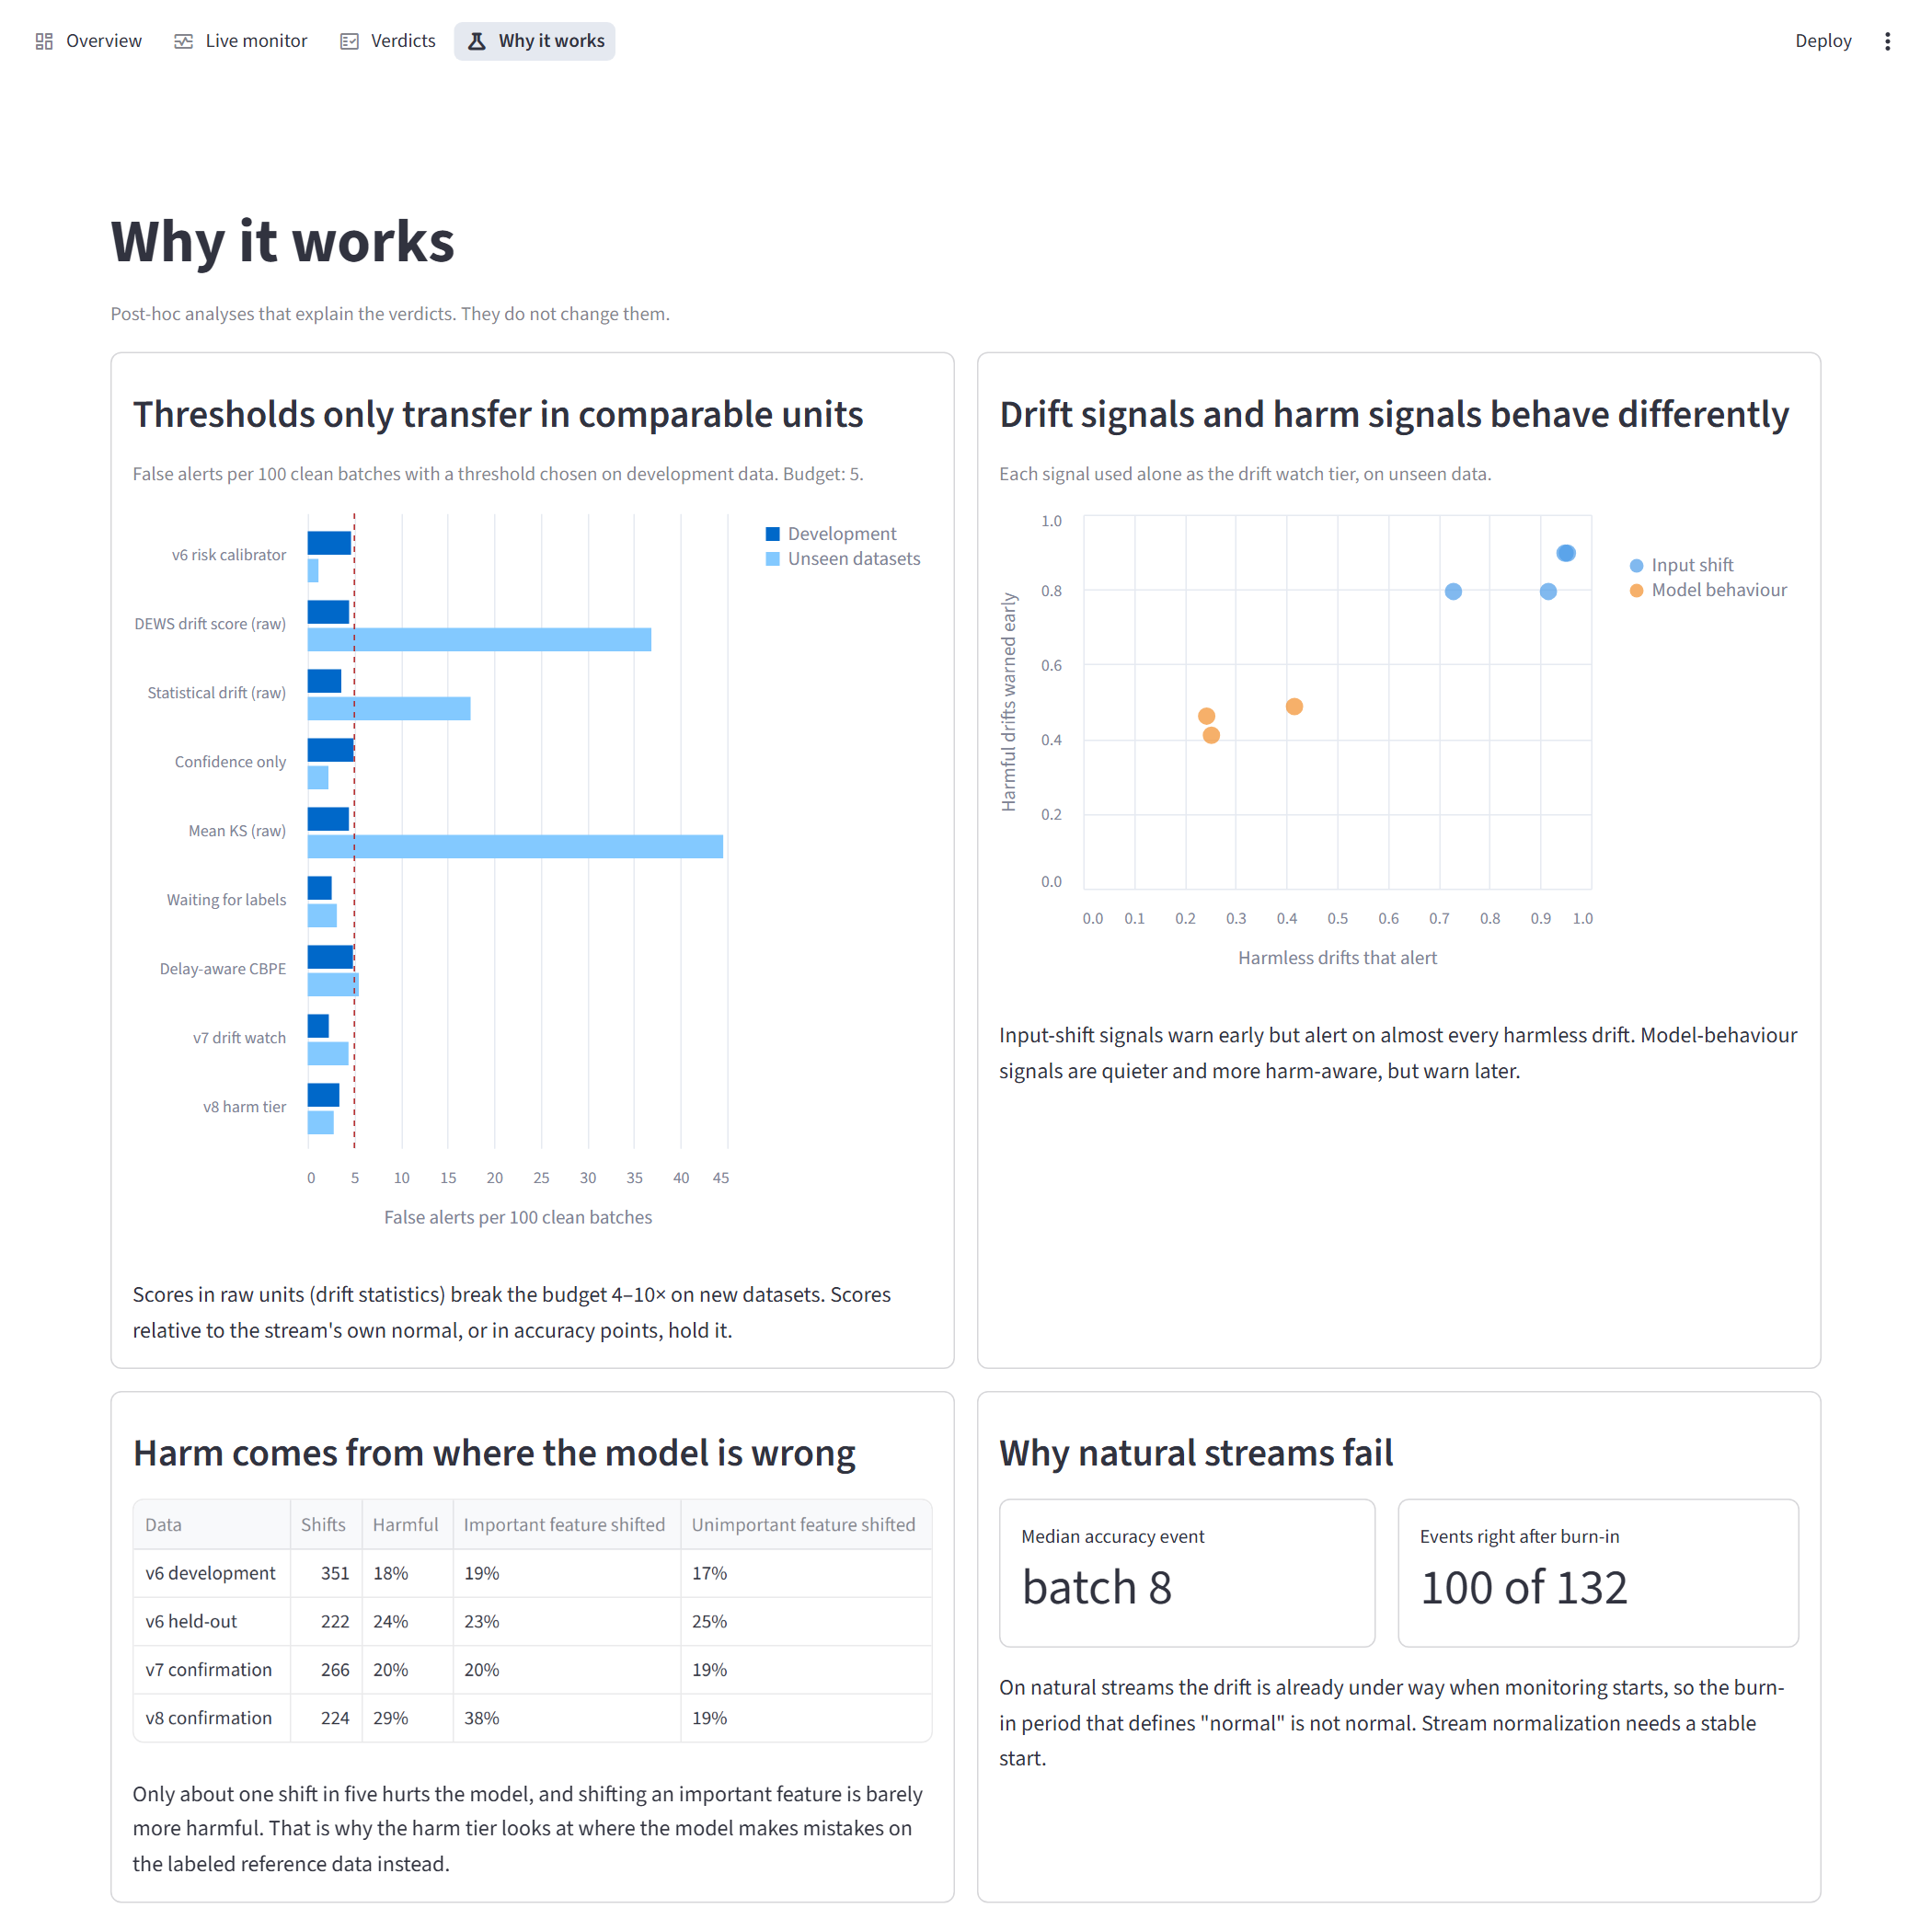
\includegraphics[width=0.85\textwidth]{ablations.png}
\caption{Dashboard: ``Why it works'' page with the ablation findings.}
\label{fig:scr_ablations}
\end{figure}

\section{Testing and Continuous Integration}
\label{sec:tests}
The repository contains 85 unit tests. They cover the protocol configuration, the event rule and warning tiers, label maturity (no score may change when unmatured labels change), the benchmark generator, signal extraction, the v7 monitor, the dashboard's data and replay logic, and components of the original prototype (detectors, alerts, forecasting, storage). The API tests of the legacy FastAPI service are skipped when that optional component is not installed.

GitHub Actions runs on every push and pull request (\figref{fig:ci}): it installs the core requirements, runs Ruff (pinned to version 0.17.4) and the full test suite on Python 3.10, 3.11 and 3.12, and then runs a benchmark gate that checks the legacy detector's lag, alert count and accuracy. In the CI run for the final code (10 November 2026) all jobs passed, with 84 tests passed and 1 skipped on each Python version.

\begin{figure}[H]
\centering
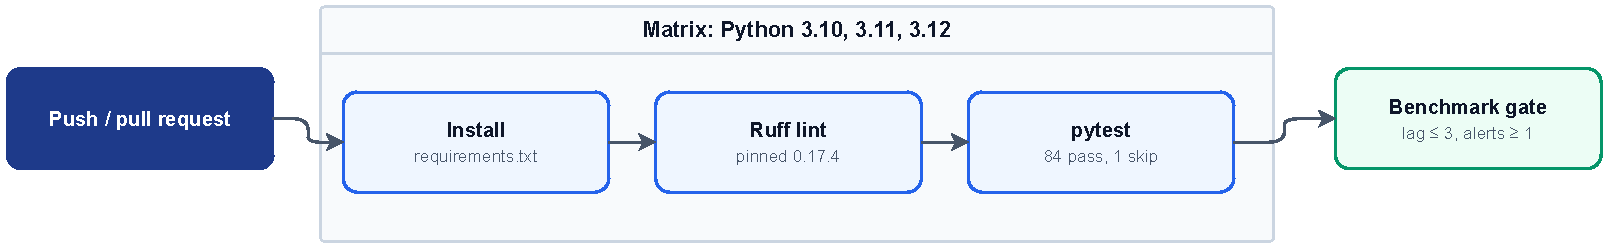
\includegraphics[width=\textwidth]{fig_ci.pdf}
\caption{Continuous-integration pipeline.}
\label{fig:ci}
\end{figure}

\section{Reproducibility}
Every episode is generated from a recorded seed, all models use fixed random states, and bootstrap intervals use fixed generator seeds. A lock file, \texttt{requirements-lock.txt}, records the exact library versions used for the frozen verdicts. The command \texttt{python scripts/reproduce.py} rebuilds whatever is missing and fails if any verdict differs from the saved one. In a clean environment, ten regenerated v8 episodes matched the saved ones to within $4\times10^{-11}$, and the v6, v7 and v8 verdicts were reproduced exactly. The v9 and v10 code is kept on separate branches of the repository because neither was adopted.

\section{Cleaning Up the Prototype}
The original repository contained a Kafka, Celery, Redis and Grafana stack and claims of production readiness that had never been evaluated. We deleted this infrastructure, since it did not help answer the research question, and rewrote the README around the measured results. The legacy FastAPI service, MLflow tracking and PostgreSQL storage were kept as optional components in a separate requirements file.
